\documentclass{beamer}

\usepackage{pgf}
\usepackage{tikz}
\usetikzlibrary{backgrounds}
\usetikzlibrary{positioning}
\usetikzlibrary{patterns}
\usetikzlibrary{decorations.pathreplacing}
\usepackage{tikzpeople}

% stolen from https://tex.stackexchange.com/questions/14225/is-there-the-easiest-way-to-toggle-show-hide-navigational-grids-in-tikz/14230
\makeatletter
\newif\if@showgrid@grid
\newif\if@showgrid@left
\newif\if@showgrid@right
\newif\if@showgrid@below
\newif\if@showgrid@above
\tikzset{%
    every show grid/.style={},
    show grid/.style={execute at end picture={\@showgrid{grid=true,#1}}},%
    show grid/.default={true},
    show grid/.cd,
    labels/.style={font={\sffamily\small},help lines},
    xlabels/.style={},
    ylabels/.style={},
    keep bb/.code={\useasboundingbox (current bounding box.south west) rectangle (current bounding box.north west);},
    true/.style={left,below},
    false/.style={left=false,right=false,above=false,below=false,grid=false},
    none/.style={left=false,right=false,above=false,below=false},
    all/.style={left=true,right=true,above=true,below=true},
    grid/.is if=@showgrid@grid,
    left/.is if=@showgrid@left,
    right/.is if=@showgrid@right,
    below/.is if=@showgrid@below,
    above/.is if=@showgrid@above,
    false,
}

\def\@showgrid#1{%
    \begin{scope}[every show grid,show grid/.cd,#1]
    \if@showgrid@grid
    \begin{pgfonlayer}{background}
    \draw [help lines]
        (current bounding box.south west) grid
        (current bounding box.north east);
%
    \pgfpointxy{1}{1}%
    \edef\xs{\the\pgf@x}%
    \edef\ys{\the\pgf@y}%
    \pgfpointanchor{current bounding box}{south west}
    \edef\xa{\the\pgf@x}%
    \edef\ya{\the\pgf@y}%
    \pgfpointanchor{current bounding box}{north east}
    \edef\xb{\the\pgf@x}%
    \edef\yb{\the\pgf@y}%
    \pgfmathtruncatemacro\xbeg{ceil(\xa/\xs)}
    \pgfmathtruncatemacro\xend{floor(\xb/\xs)}
    \if@showgrid@below
    \foreach \X in {\xbeg,...,\xend} {
        \node [below,show grid/labels,show grid/xlabels] at (\X,\ya) {\X};
    }
    \fi
    \if@showgrid@above
    \foreach \X in {\xbeg,...,\xend} {
        \node [above,show grid/labels,show grid/xlabels] at (\X,\yb) {\X};
    }
    \fi
    \pgfmathtruncatemacro\ybeg{ceil(\ya/\ys)}
    \pgfmathtruncatemacro\yend{floor(\yb/\ys)}
    \if@showgrid@left
    \foreach \Y in {\ybeg,...,\yend} {
        \node [left,show grid/labels,show grid/ylabels] at (\xa,\Y) {\Y};
    }
    \fi
    \if@showgrid@right
    \foreach \Y in {\ybeg,...,\yend} {
        \node [right,show grid/labels,show grid/ylabels] at (\xb,\Y) {\Y};
    }
    \fi
    \end{pgfonlayer}
    \fi
    \end{scope}
}
\makeatother

\begin{document}
\begin{frame}
  \frametitle{Traditional stack pointers}
  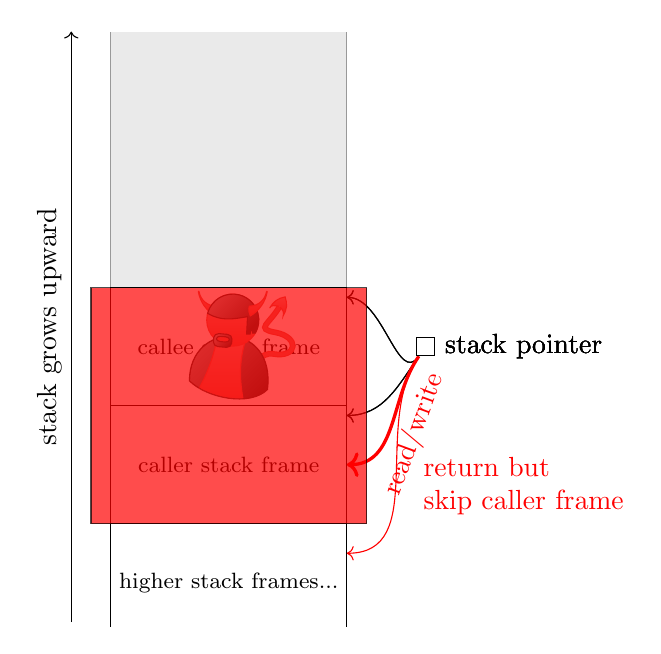
\begin{tikzpicture}[scale=.5, every node={scale=.5}]
    % recurrent parts
    \begin{scope}
      \clip (-.1,-.1) rectangle (6.1,15.1);
      \draw[fill=gray!20,draw=none,opacity=.8] (0,0) rectangle (6,15);
      \draw[draw=gray!80] (0,0) -- (0,15);
      \draw[draw=gray!80] (6,0) -- (6,15);
      \draw[fill=white] (0,-.5) rectangle (6,2.5) node[pos=.5] {\footnotesize higher stack frames...};
    \end{scope}
    \draw[->] (-1,0) -- node[midway,sloped,above] {stack grows upward} (-1,15);

    % traditional:
    \draw<+>[fill=white] (0,2.5) rectangle (6,5.5) node[pos=.5] {\footnotesize caller stack frame};
    \draw<.> (8,7) node[draw=black] (sp0) {};
    \draw<.> node[right=0cm of sp0] (sp0l) { stack pointer };
    \draw<.> (sp0) edge[->,out=235,in=0] (6,5.25);

    % traditional call:
    \draw<+>[fill=white] (0,2.5) rectangle (6,5.5) node[pos=.5] {\footnotesize caller stack frame};
    \draw<.>[fill=white] (0,5.5) rectangle (6,8.5) node[pos=.5] {\footnotesize callee stack frame};
    \draw<.> (8,7) node[draw=black] (sp0) {};
    \draw<.> node[right=0cm of sp0] (sp0l) { stack pointer };
    \draw<.> (sp0) edge[->,out=235,in=0] (6,8.25);

    % traditional return:
    \draw<+>[fill=white] (0,2.5) rectangle (6,5.5) node[pos=.5] {\footnotesize caller stack frame};
    \draw<.> (8,7) node[draw=black] (sp0) {};
    \draw<.> node[right=0cm of sp0] (sp0l) { stack pointer };
    \draw<.> (sp0) edge[->,out=235,in=0] (6,5.25);

    % traditional call, attack:
    \draw<+->[fill=white] (0,2.5) rectangle (6,5.5) node[pos=.5] {\footnotesize caller stack frame};
    \draw<.->[fill=white] (0,5.5) rectangle (6,8.5) node[pos=.5] {\footnotesize callee stack frame};
    \draw<.-> (8,7) node[draw=black] (sp0) {};
    \draw<.-> node[right=0cm of sp0] (sp0l) { stack pointer };

    % read other stack frames
    \draw<.> (sp0) edge[->,out=235,in=0] (6,8.25);
    \draw<.> (3,7) node[devil,mirrored,minimum size=1cm] {};
    \draw<.> (sp0) edge[->,color=red,very thick,out=235,in=0] node[sloped, below] {read/write} (6,4);

    % break well-bracketedness
    \draw<+>[fill=red,opacity=.7] (-.5,2.5) rectangle (6.5,8.5);
    \draw<.-> (8,7) node[draw=black] (sp0) {};
    \draw<.>[red] (sp0) edge[->,out=235,in=0] (6,1.75);
    \draw<.> node[color=red,align=left,below=of sp0l] {return but\\
      skip caller frame};
  \end{tikzpicture}

\end{frame}

\begin{frame}
  \frametitle{Stack and return capabilities}
  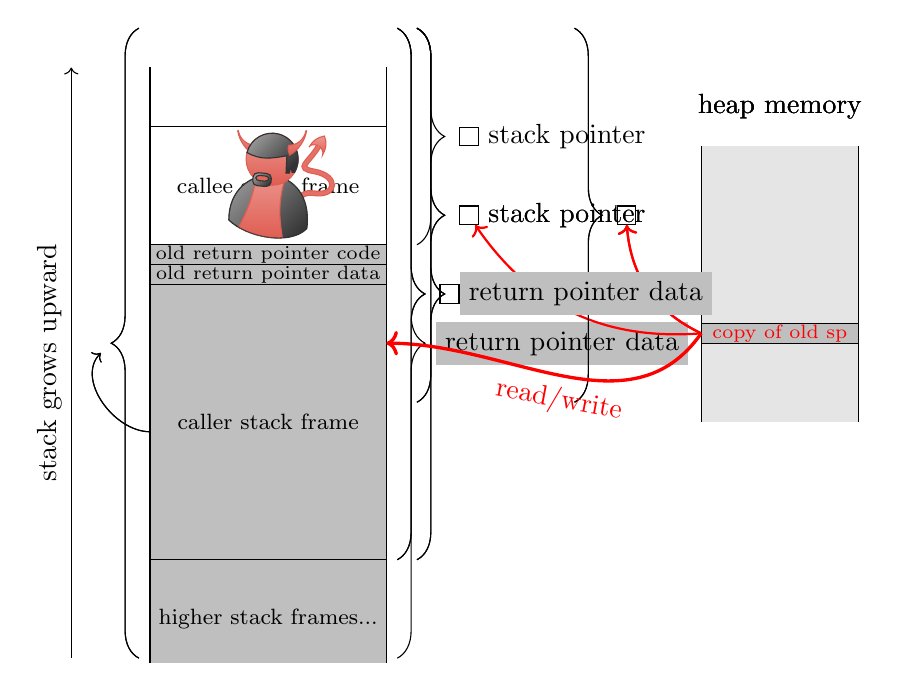
\begin{tikzpicture}[scale=.5, every node={scale=.5}]
    % recurrent parts
    \begin{scope}
      \clip (-.1,-.1) rectangle (6.1,15.1);
      \draw[fill=gray!20,draw=none,opacity=.8] (0,0) rectangle (6,15);
      \draw[draw=gray!80] (0,0) -- (0,15);
      \draw[draw=gray!80] (6,0) -- (6,15);
      \draw[fill=gray!50] (0,-.5) rectangle (6,2.5) node[pos=.5,color=black] {\footnotesize higher stack frames...};
    \end{scope}

    \draw[->] (-2,0) -- node[midway,sloped,above] {stack grows upward} (-2,15);

    % first step: capabilities
    \draw<+>[fill=white] (0,2.5) rectangle (6,5.5) node[pos=.5] {\footnotesize current stack frame};
    \begin{scope}
      \clip (-.1,-.1) rectangle (6.1,15);
      \draw<.>[fill=white] (0,5.5) rectangle (6,15.1);
    \end{scope}
    \draw<.> [decorate,decoration={brace,amplitude=10pt,mirror,raise=4pt},yshift=0pt]
    (6.5,2.5) -- (6.5,16) node[draw=black] (sp1) [black,midway,xshift=0.8cm] {};
    \draw<.> node[right=0cm of sp1] { stack pointer };
    \draw<.> [decorate,decoration={brace,amplitude=10pt,mirror,raise=4pt},yshift=0pt]
      (6,0) -- (6,16) node (oldframe1) [black,midway,xshift=0.5cm] {};
    \draw<.> node[fill=gray!50,right=0cm of oldframe1] (rp1l) {return pointer data};

    % call using capabilities
    \draw<+>[fill=gray!50] (0,2.5) rectangle (6,5.5) node[pos=.5] {\footnotesize caller stack frame};
    \draw<.>[fill=white] (0,6.5) rectangle (6,9.5) node[pos=.5] {\footnotesize callee stack frame};
    \begin{scope}
      \clip (-.1,-.1) rectangle (6.1,15);
      \draw<.>[fill=white] (0,9.5) rectangle (6,15.1);
    \end{scope}
    \draw<.> [decorate,decoration={brace,amplitude=10pt,mirror,raise=4pt},yshift=0pt]
      (6.5,6.5) -- (6.5,16) node[draw=black] (sp1) [black,midway,xshift=0.8cm] {};
    \draw<.> node[right=0cm of sp1] { stack pointer };
    \draw<.> [decorate,decoration={brace,amplitude=10pt,mirror,raise=4pt},yshift=0pt]
      (6,2.5) -- (6,16) node (callerframe1) [draw=black,midway,xshift=0.8cm] {};
    \draw<.> node[fill=gray!50,right=0cm of callerframe1] (rp1l) {return pointer data};
    \draw<.>[fill=gray!50] (0,5.5) rectangle node {\scriptsize old return pointer data} (6,6);
    \draw<.>[fill=gray!50] (0,6) rectangle node {\scriptsize old return pointer code} (6,6.5);
    \draw<.> [decorate,decoration={brace,amplitude=10pt,raise=4pt},yshift=0pt]
      (0,0) -- (0,16) node (oldframe1) [black,midway,xshift=-0.5cm] {};
    \draw<.> (0,5.75) edge[->,out=180,in=225] (oldframe1);

    % attacker...
    \draw<+>[fill=gray!50] (0,2.5) rectangle (6,5.5) node[pos=.5] {\footnotesize caller stack frame};
    \draw<.>[fill=white] (0,6.5) rectangle (6,9.5) node[pos=.5] {\footnotesize callee stack frame};
    \draw<.>[fill=gray!50] (0,5.5) rectangle node {\scriptsize old return pointer data} (6,6);
    \draw<.>[fill=gray!50] (0,6) rectangle node {\scriptsize old return pointer code} (6,6.5);
    \begin{scope}
      \clip (-.1,-.1) rectangle (6.1,15);
      \draw<.>[fill=white] (0,9.5) rectangle (6,15.1);
    \end{scope}
    \draw<.> (3,8) node[devil,mirrored,minimum size=1cm] {};
    \draw<.> [decorate,decoration={brace,amplitude=10pt,mirror,raise=4pt},yshift=0pt]
      (6.5,6.5) -- (6.5,16) node[draw=black] (sp1) [black,midway,xshift=0.8cm] {};
    \draw<.> node[right=0cm of sp1] { stack pointer };

    \begin{scope}
      \clip (13.9,6) rectangle (18.1,13);
      \draw<.>[fill=gray!20] (14,5.9) rectangle (18,13.1);
    \end{scope}
    \draw<.> (16,14) node {heap memory};
    \draw<.>[fill=gray!50] (14,8) rectangle node[color=red] {\scriptsize copy of old sp} (18,8.5);
    \draw<.> (14,8.25) edge[->,red,thick,bend left] (sp1);
    
    \begin{scope}
      \clip (13.9,6) rectangle (18.1,13);
      \draw<+>[fill=gray!20] (14,5.9) rectangle (18,13.1);
    \end{scope}
    \draw<.> (16,14) node {heap memory};
    \draw<.>[fill=gray!50] (14,8) rectangle node[color=red] {\scriptsize copy of old sp} (18,8.5);
    \draw<.> [decorate,decoration={brace,amplitude=10pt,mirror,raise=4pt},yshift=0pt]
      (10.5,6.5) -- (10.5,16) node[draw=black] (spold) [black,midway,xshift=0.8cm] {};
    \draw<.> (14,8.25) edge[->,red,thick,bend left] (spold);
    \draw<.> [decorate,decoration={brace,amplitude=10pt,mirror,raise=4pt},yshift=0pt]
    (6.5,2.5) -- (6.5,16) node[draw=black] (sp1) [black,midway,xshift=0.8cm] {};
    \draw<.> node[right=0cm of sp1] { stack pointer };
    \draw<.>[fill=white] (0,2.5) rectangle (6,5.5) node[pos=.5] {\footnotesize current stack frame};
    
    \begin{scope}
      \clip (13.9,6) rectangle (18.1,13);
      \draw<+>[fill=gray!20] (14,5.9) rectangle (18,13.1);
    \end{scope}
    \draw<.> (16,14) node {heap memory};
    \draw<.>[fill=gray!50] (14,8) rectangle node[color=red] {\scriptsize copy of old sp} (18,8.5);
    \draw<.> [decorate,decoration={brace,amplitude=10pt,mirror,raise=4pt},yshift=0pt]
      (10.5,6.5) -- (10.5,16) node[draw=black] (spold) [black,midway,xshift=0.8cm] {};
    \draw<.> (14,8.25) edge[->,red,thick,bend left] (spold);
    \draw<.>[fill=gray!50] (0,2.5) rectangle (6,9.5) node[pos=.5] {\footnotesize caller stack frame};
    \draw<.>[fill=white] (0,10.5) rectangle (6,13.5) node[pos=.5] {\footnotesize callee stack frame};
    \draw<.> (3,12) node[devil,mirrored,minimum size=1cm] {};
    \draw<.> (14,8.25) edge[->,color=red,very thick,out=235,in=0] node[sloped, below] {read/write} (6,8);
    \begin{scope}
      \clip (-.1,-.1) rectangle (6.1,15);
      \draw<.>[fill=white] (0,13.5) rectangle (6,15.1);
    \end{scope}
    \draw<.> [decorate,decoration={brace,amplitude=10pt,mirror,raise=4pt},yshift=0pt]
      (6.5,10.5) -- (6.5,16) node[draw=black] (sp1) [black,midway,xshift=0.8cm] {};
    \draw<.> node[right=0cm of sp1] { stack pointer };
    \draw<.> [decorate,decoration={brace,amplitude=10pt,mirror,raise=4pt},yshift=0pt]
      (6,2.5) -- (6,16) node (callerframe1) [draw=black,midway,xshift=0.8cm] {};
    \draw<.> node[fill=gray!50,right=0cm of callerframe1] (rp1l) {return pointer data};
    \draw<.>[fill=gray!50] (0,9.5) rectangle node {\scriptsize old return pointer data} (6,10);
    \draw<.>[fill=gray!50] (0,10) rectangle node {\scriptsize old return pointer code} (6,10.5);
    \draw<.> [decorate,decoration={brace,amplitude=10pt,raise=4pt},yshift=0pt]
      (0,0) -- (0,16) node (oldframe1) [black,midway,xshift=-0.5cm] {};
    \draw<.> (0,5.75) edge[->,out=180,in=225] (oldframe1);
    
  \end{tikzpicture}
\end{frame}
\end{document}